\section{Elektrische Netze}
%Text

\subsection{Leitungen}

\subsubsection{Leitungsbeläge}
Bisher haben wir die Grundlagen der Gleich- beziehungsweise Wechselstromtechnik im Allgemeinen kennen gelernt.
Insbesondere bei der Betrachtung von Blindleistungen geht man dabei meist davon aus,
dass ein Verbraucher durch den Einsatz von Spulen oder Kondensatoren Blindleistung erzeugt.
Wir interessieren uns jedoch für die Energienetze und hier kommt ein wichtiger Punkt hinzu:
Auch die Leitungen selbst haben einen Widerstand, eine Kapazität, eine Induktivität, sowie die noch einzuführende Ableitung.
Diese bezeichnet man auf die Länge bezogen als Widerstand-, Kapazitäts-, Induktivitäts- und Ableitungsbeläge und fasst sie unter dem Begriff der Leitungsbeläge zusammen.

Zunächst sei noch die Ableitung eingeführt: Die Ableitungsbeläge beschreiben die Verluste durch unvollständige Isolation des Leiters. Die Ableitung wird in Siemens gemessen\footnote{Eine alternative, ältere Bezeichnung für das Siemens ist das Mho (Ohm rückwärts gelesen) $\mho$ }, was den Kehrwert der Einheit Ohm darstellt:
\begin{equation}
\mathrm{[S]} = \frac{1}{\Omega} = \frac{A}{V}
\end{equation}
und die Ableitungsbeläge folglich in Siemens pro Meter.
Die Ableitung ist dank moderner Isolationstechnik deutlich geringer als die Ohmschen Verluste.

Bei der Betrachtung der Leitungsbeläge und der daraus folgenden Anforderungen an die Leitungen muss man zwischen drei unterschiedlichen Leitungstypen unterscheiden: Freileitungen, Erdkabel und Seekabel.

\subsubsection{Freileitungen}
Der überwiegende Teil der Hochspannungs-Energieverteilung geschieht mit Freileitungen.
Dabei werden nicht isolierte Leiterseile an Isolatoren an etwa 50 Meter hohen und etwa 400 Meter voneinander entfernten Hochspannungsmasten aufgehängt. % Werte für GB
In Deutschland gibt es Freileitungen mit Spannungen von bis zu 380 kV, in anderen Ländern auch bis 1000 kV und Anlagen mit bis zu 2 MV sind geplant\cite{Flosdorff}.
Es gibt unterschiedliche Arten und Bauweisen von Freileitungsmasten, auf die wir hier nicht näher eingehen wollen. Wichtig sind für uns lediglich die sich dadurch ergebende Anzahl und Anordnung der Leiterseile, deren Bodenhöhe und Abstand zu einander.

\begin{figure}[tbhn]
\begin{center}
\noindent
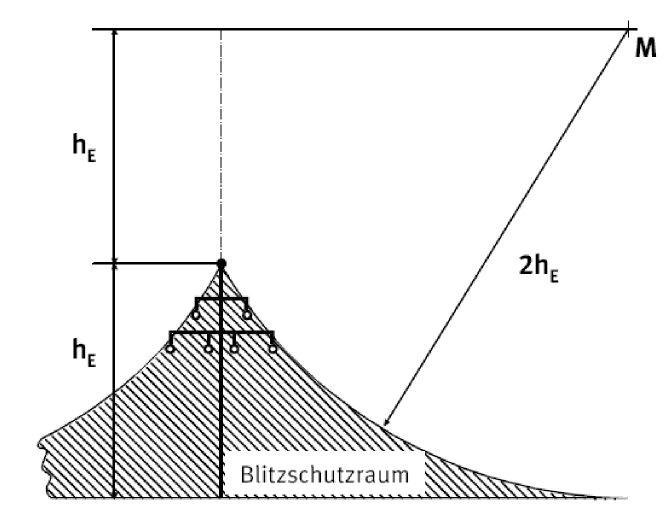
\includegraphics[scale=0.8]{blitzschutzraum.png}
\end{center}
\caption{Blitzschutzraum einer Freileitung. Quelle: \cite{Harnischmacher} verwendetin \cite{BfN}} %mehr
\label{pic:blitzschutzraum}
\end{figure}

Die Spitzen der Masten tragen ein Erdseil, welches die Leiterseile vor Blitzschlag schützen, indem sie einen Schutzraum bilden. Er wird näherungsweise durch den Zwischenraum zwischen zwei den Boden und das Erdseil tangierenden Kreisen mit doppelter Masthöhe als Radius beschrieben. Die Masten sind derartig gebaut, dass die Leiterseile sich in diesem Schutzraum befinden. Um bei – im Fall von besonders hohen Spannungen nötigen – weiten Traversen den Mast nicht zu hoch bauen zu müssen, kann man auch durch Verwendung von zwei statt nur einem Erdseil den Schutzraum vergrößern.

Bei den Leiterseilen handelt es sich meist um Verbundseile mit einem Kern aus Stahl, der die mechanische Stabilität gewährleistet, umgeben von Aluminiumleitern. Aluminium hat zwar im Bezug auf das Volumen einen höheren Widerstand als Kupfer, im Bezug auf das Gewicht leitet Aluminium hingegen besser. Ein typisches 650-A-Leiterseil besteht aus 7 Stahl- und 54 Aluminiumadern, die jeweils einen Durchmesser von 3 mm haben.\cite{Harrison}.
Moderne Leiterseile bestehen oft ganz aus einer Aluminiumlegierung und haben dadurch einen höheren Stromtragefähigkeit, einen geringen ohmschen Widerstand und müssen weniger gewartet werden\cite{Harrison}.
%% Skineffekt

Bei höheren Spannungen verwendet man statt einem dicken mehrere dünnere Leiterseile pro Leiter in geringem Abstand. Dadurch sind die Randfeldstärken\footnote{Die Randfeldstärke darf zur Vermeidung von Koronaentladung nicht größer als 17 kV/cm werden.\cite{Flosdorff}} und die Induktivität geringer und durch die bessere Kühlung aufgrund der größeren Oberfläche kann ein größerer Strom geführt werden. Man spricht hier von Bündelleitern.
Seit einigen Jahren stattet man vor allem die Erdseile, aber auch die Leiterseile mit Lichtwellenleitern zur Datenübertragung aus. Diese dienten zunächst der innerbetrieblichen Fernüberwachung und -steuerung, wird heute jedoch vor allem auch für privat genutzte Telefonnetze verwendet.\cite{Flosdorff}
% Durchhang, entfernung, Last, Wetter, etc. ?

\begin{figure}[tbhn]
\begin{center}
\noindent
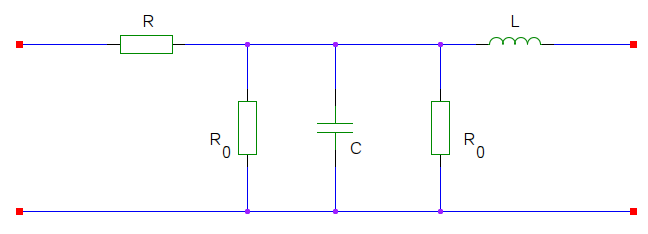
\includegraphics[scale=0.5]{freileitung.png}
\end{center}
\caption{Ersatzschaltbild einer Freileitung} %mehr
\label{pic:Ersatzschaltbildfreileitung}
\end{figure}

In Abbildung \ref{pic:Ersatzschaltbildfreileitung} ist ein Ersatzschaltbild für eine einphasige Leitung mit den Leitungsbelägen gezeichnet.
% Alternativ: π-Glied
Dabei ist $R$ der serielle Widerstand, $L$ die serielle Induktivität, $C$ die parallele Kapazität und $R_0$ der Ableitungswiderstand. Für die genaue Betrachtung muss man sich dieses infinitesimal klein unendlich oft hintereinander geschaltet vorstellen, für kurze Leitungen (unter 100 km Länge) kann man es jedoch näherungsweise auf eine derartige Schaltung reduzieren\cite{Harrison}.
Außerdem sind im allgemeinen die Induktivitäten nicht notwendigerweise zeitlich konstant\cite{Flosdorff}.
Typische Werte für den Widerstand, die Induktivität und Kapazität findet man in Tabelle \ref{tab:freileitung}.
Der Ableitungsbelag setzt sich bei Freileitungen zusammen aus den sogenannten Leckströmen, die über die Isolatoroberflächen abfließen, und den Verlusten durch die Koronaentladung zusammen.\cite{Heuck}
Der Wert für die Ableitungsbelag hängt stark von äußeren Faktoren, wie den Umgebungsbedingungen und dem Verschmutzungsgrad der Isolatoren ab. Ein typische Wert ist $200\,M\Omega m^{-1}$.\cite{Harrison} Die Ableitungsverluste sind also meist deutlich geringer als die seriellen ohmschen Verluste, weshalb man sie in den meisten Betrachtungen ignorieren kann.
Wie wir sehen ist eine Freileitung weitgehend induktiv. % sieht man garnicht

\setlength{\tabcolsep}{10pt}
\renewcommand{\arraystretch}{1.5}
\begin{table}[tbhn]
\begin{center}
\noindent
\begin{tabular}{|c|ccc|}
\hline 
Leitung & 132 kV ($1\cdot 175\ mm^2$) & 275 kV ($2\cdot 400\ mm^2$) & 400 kV ($4\cdot 400\ mm^2$) \\ 
\hline 
R & 0,178 $\Omega$ & 0,039 $\Omega$ & $0,02 \Omega$ \\ 

$X_L$ & 0,40 $\Omega$ & 0,32 $\Omega$ & 0,278 $\Omega$ \\ 

$X_C$ & 350 k$\Omega$ & 275 k$\Omega$ & 245 k$\Omega$ \\ 
\hline 
\end{tabular} 
\end{center}
\caption{Typische Leitungsbeläge von drei verschiedenen Leitungen. Quelle: \cite{Harrison}} %fehlt
\label{tab:freileitung}
\end{table}

%%% Induktivität %%%
\paragraph{Induktivitätsbelag}

Fließen Wechselströme durch mehrere nebeneinander liegende Leiter so wird durch Selbstinduktion und Gegeninduktion eine Wechselspannung induziert.

%bla, von wegen kan als selbstinduktion gesehen werden
Die Induktivität eines Leiters $v$ hängt wie folgt mit dm magnetischem Fluss an dessen Position zusammen:
\begin{equation}
L_v = N_v \frac{\Phi_v}{i_v}
\end{equation}
Laut \cite{Flosdorff}\cite{Moeller} % besser [42] dort
ist $N_v = 1$, somit müssen wir um die Induktivität zu berechnen den magnetischen Fluss berechnen, welchen sich aus den Flüssen aller Leiter zusammensetzt. Es gilt also das Gleichungssystem:
\begin{equation}\label{eq:SummePhi}
\Phi_v = \sum_k \Phi_{vk}
\end{equation}
%Da Feldlinien stets von einer Quelle ausgehen und in einer Senke enden, benötigen wir noch eine äußere Feldbegrenzung. %realy?
Zur Berechnung der Flüsse führen wir einen Zylinder mit sehr großem, aber endlichem Radius $r_a$ und den Leiter $v$ als Mittelpunkt als Feldbegrenzung ein. Die Rechtfertigung dafür werden wir später sehen.
Der Fluss den der Leiter selbst erzeugt ist laut \cite{Moeller}\cite{Flosdorff} % beide zitieren?
\begin{equation}
\Phi_{vv} = \frac{\mu_0l}{2\pi} \left( \ln\frac{r_a}{r_v} + 0,25 \right) i_v
\end{equation}
Der Fluss im Leiter $v$ der von einem Leiter $k$ erzeugt wird ist das Integral des Magnetfelds über die Fläche zwischen Leiter und Begrenzungszylinder:
\begin{equation}
\Phi_{vk} = \int_A B_k dA = \int\limits_{x=d_{vk}}^{x=r_a} \frac{\mu_0i_k l}{2\pi x}dx =
\frac{\mu_0l}{2\pi}\ln\left(\frac{r_a}{d_{vk}}\right) i_k
\end{equation}
Setzt man dies in Gleichung \ref{eq:SummePhi} ein, so erhält man:
\begin{equation}
\Phi_v = \frac{\mu_0l}{2\pi} \left[ \left( \ln\frac{r_a}{r_v} +0,25\right) i_v + \sum_{k\neq1}\ln\frac{r_a}{d_{vk}} i_k \right]
\end{equation}
Wir beziehen den Fluss auf die Länge der Leitung und zeihen $r_a$ raus:
\begin{equation}
\Phi'_v = \frac{\mu_0}{2\pi}
 \left[
   \ln r_a \sum i_k +
   \sum_k \left( \ln\frac{1}{d_{vk}} i_k +
   0,25 \: \delta_{ik} \right)
 \right]
\quad mit \: d_{v1}:=r_v
\end{equation}
Die Summe aller Leiterströme muss immer null sein $\sum i_k=0$ und somit verschwindet der erste Term und die Gleichung ist unabhängig von $r_a$. Das Gleichungssystem für die Flüsse wird somit zu:
\begin{equation}
\Phi'_v = \sum_k a_{vk}i_k
\end{equation}
mit den Koeffizienten:
\begin{equation}
a_vv = \frac{\mu_0}{2\pi} \left( \ln\frac{1}{r_v} + 0,25 \right) \qquad und \qquad a_{vk} = a_{kv} = \frac{\mu_0}{2\pi} \ln\frac{1}{d_{ik}}
\end{equation}
Betrachten wir zunächst ein \textbf{Zweileitersystem}. Das obige Gleichungssystem reduziert sich auf:
\begin{align}
\Phi'_1 &= a_{11}i_1 + a_{12}i_2 \\
\Phi'_2 &= a_{21}i_i + a_{22}i_2
\end{align}
Dabei ist $i_2 = -i_1$ und $d_{12} = d_{21} = d$. Die Induktivität errechnet sich nun einfach zu:
\begin{equation}
L'_1 = a_{11} - a{12} = \frac{\mu_0}{2\pi}\left(\ln\frac{1}{r_1}+025\right)-\frac{\mu_0}{2\pi}\ln\frac{1}{d} = 
\frac{\mu_0}{2\pi}\left(\ln\frac{d}{r_1}+025\right)
\end{equation}
und gleichfalls für Leiter 2. In der Regel sind die beiden Leiterradien gleich, wodurch beide Leiter die selbe Induktivität haben – was aus Symmetriegründen selbst verständlich war. Will man die Induktivität nicht auf die Leiterlänge sonder auf die Leitungslänge beziehen, so muss man die Induktivität verdoppeln, da man zwei Leiter hat – man erhält also schließlich:
\begin{equation}
L' = \frac{\mu_0}{\pi}\left(\ln\frac{d}{r_1}+025\right)
\end{equation}

\begin{figure}[bthn]
\begin{center}
\noindent
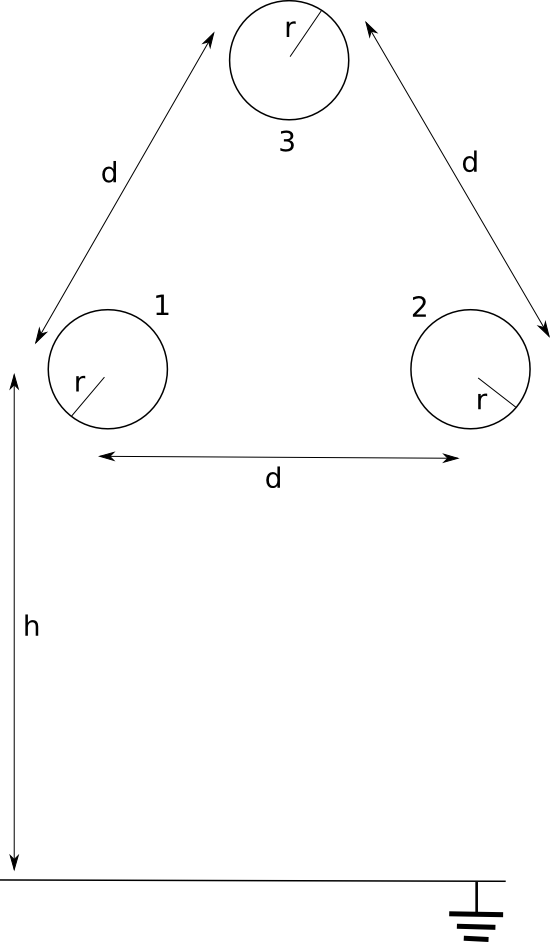
\includegraphics[scale=0.3]{leitungsreaktanz.png}
\end{center}
\caption{Skizze zur Berechnung des Induktivitätsbelags einer Freileitung mit symmetrische Dreileiteranordnung} 
\label{pic:leitungsreaktanz} 
\end{figure}

Ein weiterer wichtiger Sonderfall ist die \textbf{symmetrische Dreileiteranordnung}, bei welcher alle drei Leiterabstände sowie Leiterradien jeweils gleichgroß sind: $d_1=d_2=d_3:=d$ und $r_1=r_2=r_3:=r$ und somit $a_{12}=a_{23}=a_{13}$ (vergleiche Abb. \ref{pic:leitungsreaktanz}). Auch hier sind die Induktivitäten der Leiter gleich groß. Wir errechnen für den ersten Leiter:
\begin{equation}
\Phi'_1 = a_{11}i_1+a_{12}i_2+a_{13}i_3 = a_{11}i_1+a_{12}\left(i_2+i_3\right) = \left(a_{11}-a_{12}\right)i_1
\end{equation}
und daraus:
\begin{equation}
L'_1 = \frac{\Phi'_1}{i_1} = a_{11}-a_{12} = \frac{\mu_0}{2\pi}\left(\ln\frac{1}{r}+0,25-\ln\frac{1}{d} \right) =
\frac{\mu_0}{2\pi}\left(\ln\frac{d}{r}+0,25 \right)
\end{equation}
Ist das Drehstromnetz gleichphasig belastet, so addieren sich die Spannungen und Ströme zu null und es genügt einphasig zu rechnen, da keine Rückführung mehr nötig ist. Die auf die Leitungslänge gerechnete Induktivität ist also:
\begin{equation}\label{eq:Induktivitaet3}
L' = L'_1 = \frac{\mu_0}{2\pi}\left(\ln\frac{d}{r}+0,25 \right)
\end{equation}
Laut \cite{Harrison} gilt diese Gleichung nur für $h\gg d$ – ist dies nicht gegeben, muss man Einflüsse des Bodens berücksichtigen.

Sind die Leiter nicht symmetrisch mit gleichen Leiterabständen angeordnet, so ergeben sich für die unterschiedlichen Leiter unterschiedliche Induktivitäten. Da dies im Allgemeinen unerwünscht ist, verdrillt man die Leiter: man wechselt die Positionen periodisch, so das jedes Kabel einmal jede der drei Positionen eingenommen hat. Dadurch gleichen sich die unterschiedlichen Induktivitäten in der Leiter aus und es gilt Gleichung \eqref{eq:Induktivitaet3} mit dem geometrischem Mittelwert der Leiterabstände
\begin{equation}
\bar{d} = \sqrt[3]{d_{12}d_{23}d_{31}}
\end{equation}
anstatt $d$.
%% Vereinfachung
%% Formel für Last

%%% Berechnung Kapazität %%%
\paragraph{Kapazitätsbelag}
\begin{figure}[tbhn]
\begin{center}
\noindent
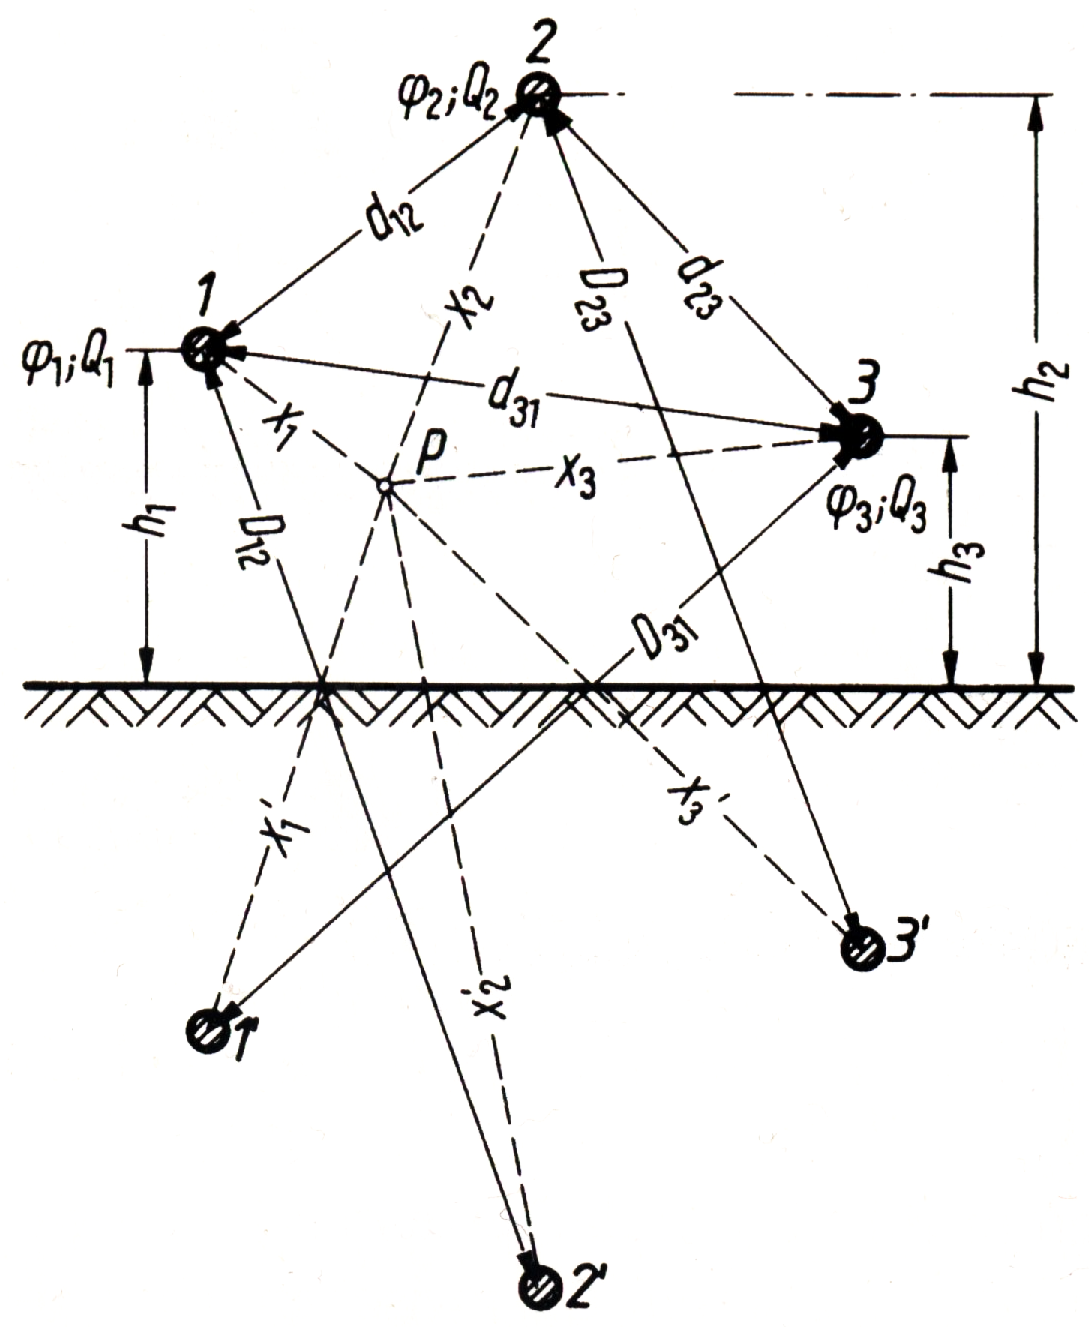
\includegraphics[scale=1]{gespiegelterdrehstrom.png}
\end{center}
\caption{Zur Berechnung des Kapazitätsbelags betrachten wir virtuelle Spiegelladungen. Quelle: \cite{Flosdorff}} %fehlt
\label{pic:gespiegelterdrehstrom} 
\end{figure}

 Die Kapazität einer Freileitung entsteht durch die die unterschiedlichen Potentiale der Leiterseil gegeneinander und gegenüber dem Erdpotential. Die Potentialunterschiede führen zu einem Elektrischem Feld, bestehend aus den elektrischen Flüssen $\Psi_{ij}$ zwischen zwei Leiterseilen, sowie den Flüssen $\Psi_{i0}$ zwischen je einem Leiter und dem Erdpotential. Zu jedem dieser Elektrischen Flüsse gehört eine Kapazität (Teilkapazität), welche zusammen die Kapazität der Freileitung ergeben.
Wir betrachten zunächst nur einen Leiter. Zur Berechnung der Kapazität verwenden wir Spiegelladungen: Wir ersetzen den Grund durch eine an der Erdoberfläche gespiegelte Ladung mit entgegengesetzter Ladung $Q'_1 = - Q_1$, ohne das sich das Feld ändert. Nun können wir das Potential in einem beliebigen Punkt P Als Summe der Potentiale schreiben:
\begin{equation}
\varphi = \frac{Q_1}{2\pi\varepsilon_0} \int^{x_1}_{r_1} \frac{dx_1}{x_1} + \varphi_1 + \frac{Q'_1}{2\pi\varepsilon_0} \int^{x_1}_{r_1} \frac{dx'_1}{x'_1} + \varphi'_1
\end{equation}
Wobei $r_1$ der Radius der Leiter ist, welche wir im folgenden als klein im Vergleich zu den Leiterabständen betrachten. Mit $Q'_1 = - Q_1$ und $\varphi'_1 = - \varphi_1$ ergibt sich:
\begin{equation}\label{eq:einleitungsfeld}
\varphi = \frac{Q_1}{2\pi l\varepsilon_0} \ln \frac{x'_1}{x_1}
\end{equation}
An der Oberfläche des Leiters ist das Potential somit näherungsweise:
\begin{equation}
\varphi^* = \frac{Q_1}{2\pi l\varepsilon_0} \ln \frac{2h_1}{r_1}
\end{equation}
Dies entspricht aus auf Grund der Stetigkeit des Potentials % echt?
dem Potential des Leiters $\varphi_1 = \varphi^*$.
Betrachten wir nun ein System mit mehreren Leitern. Das Potential an einem wieder frei gewähltem Punkt P berechnet sich als die Summe der nach \eqref{eq:einleitungsfeld} berechneten Potentiale:
\begin{equation}
\varphi = \sum \frac{Q_i}{2\pi l\varepsilon_0} \ln \frac{x'i}{x_i}
\end{equation}
Wie zuvor setzen wir die Ortskoordinaten der Leiteoberflächen ein um die Potentiale der Leiter zu bestimmen, dadurch erhalten wir:
\begin{align}
\varphi_1 &= a_{11} Q_1 + a_{12} Q_{2} + ... + a_{1n} Q_n \\
\varphi_2 &= a_{21} Q_1 + a_{22} Q_{2} + ... + a_{2n} Q_n \\
\vdots \\
\varphi_n &= a_{n1} Q_1 + a_{n2} Q_{2} + ... + a_{nn} Q_n
\end{align}
mit den Koeffizienten
\begin{equation}
a_{ii} = \frac{\ln 2h_i/r_i}{2\pi l \varepsilon_0} \quad \textrm{und} \quad a_{ik} = \frac{\ln D_{ik}/d_{ik}}{2\pi l \varepsilon_0}
\end{equation}
Das obige Gleichungssystem muss nun nach den $Q_i$ aufgelöst werden. Das Gleichungssystem lässt sich auch in Matrizenschreibweiße $\boldsymbol{\varphi} = \uuline{A} \cdot \mathbf{Q}$ darstellen, dann entspricht das Auflösen der Invertierung der Matrix $\uuline{A}$: $\uuline{D}=\uuline{A}^{-1}$. Man erhält also allgemein:
\begin{equation}
Q_i = \sum_k d_{ik}\varphi_k
\end{equation}
Wir ziehen das Element mit $k=i$ aus der Summe hinaus und ergänzen:
\begin{equation}
Q_i = \sum_{k\neq i} d_{ik}\varphi_k + d_{ii}\varphi_i + \textcolor{blue}{\sum_k d_{ik}\varphi_i} - \textcolor{blue}
{\sum_k d_{ik}\varphi_i}
\end{equation}
Durch umsortieren und ausklammern erhalten wir schließlich eine Form in welcher wir die Teilkapazitäten identifizieren können.
\begin{equation}
Q_i = \underbrace{\left(d_{ii}+\sum_{k\neq i}d_{ik}\right)}_{:=C_{i0}}\varphi_i + \sum_{k\neq i} \underbrace{d_{ik}}_{:=C_{ik}} \left( \varphi_k - \varphi_i \right)
\end{equation}
Mithilfe der Regeln zur Parallel- und Reihenschaltung von Kondensatoren lässt sich daraus der Gesamtkapazitätsbelag berechnen.
Für eine Wechselstromleitung mit zwei Leiterseilen erhält man gemäß dieser Vorgehensweise\footnote{Dabei schrumpft das Gleichungssystem jedoch auf zwei Gleichungen zusammen, weshalb die Auflösung sehr einfach wird.}
\begin{equation}
C' = \frac{C}{l} = \frac{\varepsilon_0\pi}{\ln{\frac{2hd}{r\sqrt{\left(2h\right)^2+d^2}}}}
\end{equation}
Für eine Dreiphasenleitung ohne Erdleiter kann man man die Herleitung vereinfachen indem man ausnützt, dass die Ladungen der drei Leitungen zusammen immer Null ergeben. Möchte man jedoch, z. Bsp. für  Erdschlussstromberechnungen nicht nur die Gesamtkapazität sondern auch die einzelnen Teilkapazitäten berechnen, geht man nach dem beschriebenen Ansatz vor.
Da die Koeffizienten $a_{ii}$ und somit auch die Koeffizienten $d_{ik}$ von der Höhe der Leitungen über dem Erdboden abhängen, ergibt sich -- im Gegensatz zur Induktivität -- bei einer symmetrischen Dreiecksanordnung wie oben %verwais
unterschiedliche Kapazitäten für die Leitungen. Daher verdrillt man auch derartige symmetrische Leiter. Für einen derartigen Leiter erhält man den Kapazitätsbelag
\begin{equation}\label{eq:verdrillteindukt}
C' = \frac{2\pi\varepsilon_0}{\ln\left(2 \bar{h}\bar{d}/(r\bar{D})\right) } \approx
\frac{2\pi\varepsilon_0}{\ln\left(\bar{d}/r\right)}
\end{equation}
Wobei $\bar{h}$, $\bar{d}$ und $\bar{D}$ die geometrischen Mittelwerte der Leiterhöhen, -Abstände und der Abstände zwischen einer Leitung und einer anderen \q Spiegelleitung\q : % Anführungszeichen fixen
\begin{equation}
\bar{h} := \sqrt[3]{h_1h_2h_3}, \quad \bar{d} := \sqrt[3]{d_{12}d_{23}d_{31}} \quad \bar{D} := \sqrt[3]{d_{12'}d_{23'}d_{31'}} \approx 2\bar{h}
\end{equation}
Man kann zeigen, dass ein zusätzliches Erdseil die Erdkapazität erhöht und die die Leiterkapazität verringert, so dass die Gesammtkapaziät unverändert bleibt und Gleichung \eqref{eq:verdrillteindukt} bleibt gültig.\cite{Flosdorff}


\subsubsection{Kabel}
In urbanen Gegenden sowie in Gegenden mit besonders erhaltenswerten Landschaften, setzt man statt Freileitungen auf unter der Erde verlegt Kabel. Die Leiter sind in der Regel aus Kupfer oder Aluminium und mit Ölimpregniertem Ölband oder neuer mit speziellen Kunststoffen isoliert. % flüssigkeitsimprägniertem Polypropylen/Papier-Laminat isoliert.
Neben Kosten und Gewichtseinsparungen haben moderne Kunststoffisolierungen auch elektrische Vorteile, so haben Kabel mit flüssigkeitsimprägniertem Polypropylen/Papier-Laminat eine um 67\% niedrigere dielektrische Verluste und eine 20\% niedrigere Permittivität und somit Kapazität.\cite{Harrison} Dadurch lässt sich mehr Leistung übertragen und es muss weniger Blindleistung bereitgestellt werden.
%Gaskablenm Druckgaskabel, (Druck-)Ölkabel
PVC-Kabel werden in Niederspannungs- und Mittelspannungsnetzen bis 10 kV eingesetzt. Für Hochspannungsnetze ist es wegen der hohen dielektischen Verluste ungeeignet, hier kommen neben Ölkabeln und Druckgaskabeln neuerdings Kabel mit vernetztem Polyäthylen (VPE) zum Einsatz. VPE hat hervorragende dielektrische und thermische Eigenschaften, weshalb es immer mehr in den Mittel und Niederspannungsbereich vordringt.\cite{Flosdorff}

\begin{figure}[tbhn]
\begin{center}
\noindent
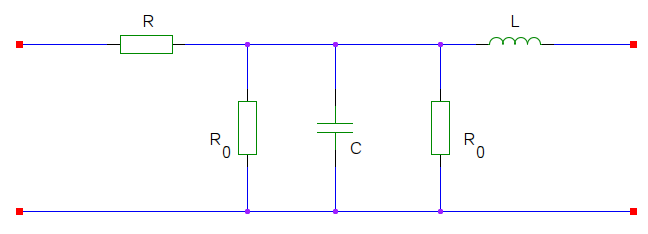
\includegraphics[scale=0.5]{kabel.png}
\end{center}
\caption{Ersatzschaltbild eines Kabels} %mehr
\label{pic:Ersatzschaltbildkabel}
\end{figure}

\begin{table}
\begin{center}
\begin{tabular}{|c|c|c|c|}
\hline 
Leitung & 132 kV ($350 mm^2$) & 275 kV ($1.000 mm^2$) & 400 kV ($2.000 mm^2$) \\ 
\hline 
Stromtragfähigkeit & 730 A & 1.090 A & 1.195 A \\ 
$C$ & 0,391 \tmu F/km & 0,368 \tmu F/km  & 0,377 \tmu F/km \\ 
Ladestrom & 9,36 A/km & 18,4 A/km & 27,4 A/km \\ 
\hline 
$L$ & \multicolumn{2}{|c|}{} & 0,4 mH \\
$R$ &  \multicolumn{2}{|c|}{} & 9 m\tOmega \\
$R_d$ & \multicolumn{2}{|c|}{} & 3,5 M\tOmega  \\
$R_0$ & \multicolumn{2}{|c|}{} & $>30$ G\tOmega  \\
\hline
\end{tabular} 
\end{center}
\caption{Typische Leitungsbeläge von drei verschiedenen Kabeln, bei üblichen Bedingungen. Quelle: \cite{Harrison}} %fehlt
\label{tab:kabel}
\end{table}

% höhere Kosten, nidrigere Zuverlässigkeit
Das Ersatzschaltbild sieht wie das der Freileitung aus, nur das man zwei Parallel geschaltete Ableitungswiederstände betrachtet.
$R_0$ ist der Isolationswiederstand, während $R_d$ die dielektrischen Verluste beschreibt. Das sind Verluste die durch Polarisationseffekte im Dielektrikum der Kapazität entstehen.
Die Induktivitäten von Kabeln lassen sich nach den selben Gleichungen berechnen, wie die von Freileitungen, da hier Herleitung dieser ohne die Bedingung $d\gg r$ auskommt.\footnote{Dabei ist $\mu_0$ natürlich durch $\mu_r\mu_0$ – mit $\mu_r$ als der relativen Permeabilität des Materials – zu ersetzen} %was ist mit h>>d ?
Da bei Kabel die Leiterabstände deutlich kleiner sind sind auch die Induktivitäten kleiner: sie betragen nur etwas 25\% bis 30\% derWerte von Freileitungen\cite{Flosdorff}.
Die Berechnung der Kapazität von Kabeln, insbesondere Gürtelkabeln, ist ungleich schwieriger als bei Freileitern, da wir vorausgesetzt haben, dass $d\gg r$ ist auserdem sind die Dielektriken und der kreisförmige Metallmantel rechnerisch nur näherungsweise bestimmbar. Daher werden die Kapazitäten experimentell vom Hersteller bestimmt.\cite{Flosdorff}
Typische Werte für ein einphasiges Kupferkabel findet man in Tabelle \ref{tab:kabel}.
Wie wir mit den Werten feststellen können, ist bei Kabeln die Kapazität überwiegend,
besonders stark ist dies bei Unterseekabeln ausgeprägt. % überprüfen, warum?, Werte
Dazu kommt, dass bei Unterseekabeln die Blindleistungskompensation nur schwer möglich ist.
Die hohen Kapazitäten erfordern hohe Ströme zum Laden der Kapazität (Ladeströme), welche durch den gesamten zur Verfügung gestellten Strom aufgebracht werden müssen. Dies reduziert die übertragbare Leistung und führt ab einer gewissen Länge dazu, dass der maximal übertragbare Strom als Ladekapazität benötigt wird. % versteh ich selbst nur halb...
Für ein 400-kV-Kabel wie in Tabelle \ref{tab:kabel} liegt diese Länge bei 43,6 km.
Daher werden bei längeren Kabeln alle paar Kilometer % wieviel genau, besser formulieren…
Induktivitäten angeschlossen um die Blindleistung zu kompensieren.

\subsection{Netzregelung}
Elektrische Netze leiten elektrische Energie, können aber weder Energie erzeugen noch speichern.
Aufgrund der Energieerhaltung muss zu jedem Zeitpunkt exakt die gleiche Menge an Wirk- und Blindleistung in das Netz eingespeist werden, wie – einschließlich aller Verluste – verbraucht wird.
Es stellt sich daher die Frage, wie dies gewährleistet werden kann und was geschieht wenn dies für kurze Zeit nicht der Fall ist – den schließlich kann man aus unerwartete Veränderungen des Verbrauchs nicht beliebig schnell reagieren.

\subsubsection{Leistungs-Frequenz-Regelung}
Zunächst betrachten wir die Wirkleistung in einem Drehstromnetz, dass von Kraftwerken mit dampfgetriebenen Turbinen gespeist wird. Das Kraftwerk kann dabei ein Kohle-, Öl- oder Kernkraftwerk sein. \footnote{Statt diesen dampfgetriebenen Turbinen lassen sich auch Wasser- oder Windkraftwerke annehmen, lediglich Turbinenlose Kraftwerke wie Photovoltaikanlagen sind hierfür ungeeignet} % Gaskraftwerke?
Neben den Kraftwerken gibt es auch zahlreiche Drehstrommotoren auf der \q Verbraucherseite\q. % Anführungszeichen
In den Turbinen, Generatoren und Motoren rotieren Massen – darin ist Rotationsenergie gespeichert.
Steigt nur der Wirkleistungsverbrauch über die Menge an produzierter Wirkleistung, so wird die Energiedifferenz aus der Rotationsenergie der Maschinen entnommen.\cite{Harrison}
Dadurch wird deren Rotation jedoch langsamer – was zu einer Verringerung der Netzfrequenz führt.
Ist der Wirkleistungsverbrauch geringer als die Produktion, so geht die überschüssige Energie in Rotationsenergie der Maschinen über und die Netzfrequenz steigt.
In den Kraftwerken erkennt nun ein Sensor die Änderung der Frequenz und regulieren die Dampfventile entsprechend:
ist die Frequenz zu niedrig, wird mehr Dampf in die Turbinen gelassen, ist die Frequenz zu hoch, wird die Dampfzufuhr reduziert.
Man hält dadurch die Frequenz immer ungefähr konstant: in Großbritannien beträgt die Frequenz im Allgemeinen $50 \mathrm{Hz} \pm 0,05 \mathrm{Hz}$.\cite{Harrison} %Wert für Deutschland
%Details; auch in DE; alternativen?

\subsubsection{Blindleistungs-Spannungsregelung}
In einem elektrischen Netz muss nicht nur die bereitgestellte Wirkleistung gleich der produzierten sein, selbiges gilt auch für die Blindleistung.
Betrachtet man eine Last, die von einem Generator über eine Leitung mit ohmschen Widerstand und Blindwiderstand mit Leistung versorgt wird. Da auch an der Leistung eine Spannung abfällt, existiert eine Differenz zwischen der Generatorspannung und der an der Last anliegenden Spannung. Diese Differenz ist auch von der Blindleistung abhängig. Steigt also der Blindleistungsbedarf plötzlich, so steigt auch die Spannungsdifferenz und die Spannung an der Last sinkt. Dadurch sinkt wiederum der Blindleistungsbedarf – aber auch der Wirkleistungsbedarf.
Als Zahlenbeispiel sei genannt, dass eine Reduktion der Spannung um 1\% im gesamten Britischen Netz die Nachfrage nach Blindleistung um 5\% und die Nachfrage nach Wirkleistung um 1,4\% senken würde.
%Spannungsänderung duch stufensteller - was hat das damit zu tun?
%Bevor wir uns überlegen, wie dies gewährleistet wird,
Nun wollen wir ein paar Worte zur Erzeugung und "Vernichtung" von Blindleistung zum Ausgleich der von Verbrauchern und Leistungen erzeugten Blindleistung verlieren. Die wichtigste Rolle spielen dabei Synchrongeneratoren und Synchron-Phasenschieber.
Ist der Generator überangeregt, % erklären was das ist.
so erzeugt er Blindleistung, ist er unterangeregt, so nimmt der Blindleistung auf. Größe Synchrongeneratoren können bis zu 50\% ihrer Bemessungsleistung in Form von Blindstrom bereitstellen. %formulierung
Jedoch darf die aufgenommene Blindleistung nur bis zu 15\% detragen, wenn gleichzeitig die volle Wirkleistung erzeugt werden soll.\cite{Harrison}	%formulierung, so korrekt?, warum
Bei Synchron-Phasenschieber handelt es sich um im Leerlauf betriebene Synchronmotoren, deren Erregung automatisch durch die Spannung geregelt werden. Sie nehmen nur geringe Wirkleistung auf um ihre Verluste aus zu gleichen. Ein Gasturbinen-Generator kann – wenn keine Wirkleistung erzeugt werden soll – bei geeigneter Bauart von seiner Turbine abgekoppelt werden und dann als Synchron-Phasenschieber betrieben werden.\cite{Harrison}

Blindleistung kann auch durch parallelgeschaltete Kapazitäten erzeugt werden, diese haben jedoch den Nachteil das ihre Blindleistung proportional zu $U^2$ ist – sie also genau dann wenn man sie am dringendsten braucht weniger Blindleistung bereitstellen.\cite{Harrison}

\subsubsection{Gleichstrom-Netzregelung}
Die Regelung einer Gleichstromleitung ist weniger einfach, es wurden jedoch technische Möglichkeiten gefunden, eine HGÜ-Leitung äußerst schnell zu regeln. Auf diese wollen wir jedoch hier nicht eingehen, da sie eine umfangreiche Beschäftigung mit den technischen Details der Stromrichterstationen erfordern würden. % mehr

\subsection{Schalter}
Es mag zwar auf den ersten Blick trivial erscheinen, einen Schalter zu bauen, doch sind die Spannungen in Energienetzen so hoch, dass beim trennen eines Kontaktschalters eine Entladung über einen Lichtbogen auftritt, welcher gelöscht werden muss.
Neben zahlreichen technischen Tricks, wie Löschgase oder Öl, behilft man sich bei Wechselstrom-Schaltern dadurch,
dass man die Kontakte genau in dem Moment trennt in welchem die Spannungskurve einen Nulldurchlauf hat. %richttig?
Da man bei HGÜ keine Nulldurchgänge hat, ist das Bauen von leistungsfähigen Gleichstrom-Schaltern nicht möglich. %Quelle, mehr!

\subsection{Gleichstromübertragung}
Das betreiben von vermaschten Gleichstromleitungen ist bis heute kaum möglich, da es dazu leistungsfähigere Schalter bräuchte.\cite{Schymroch}
Daher sind Gleichstromleitungen bis heute auf Punkt-zu-Punkt-Verbindungen beschränkt.
Es gibt drei Arten von von Gleichspannungsleitungen.
Bei Monopolaren Leitungen, existiert nur ein Leiter – die Rückleitung geschieht über die Erde beziehungsweise bei Seekabeln das Meereswasser. Die Leitung wird meist mit einem im Bezug auf die Erde negativen Potential betrieben, was den Vorteil einer deutlich geringeren Koronaentladung bringt.\cite{Padiyar}
Bei Bipolaren Leitungen hingegen erfolgt der Stromfluss in beide Richtungen über einen Leiter, mit gewöhnlich gleicher Spannung. Bei besonders hohen Spannungen können aus jeweils mehrere Leiter verwendet werden. An beiden Enden sind je zwei gleichartige Konverter, auf mindestens einer Seite ist die Verbindung der beiden Konverter geerdet, auch wenn die im symmetrischem Regelbetrieb nicht für den Stromrückfluss gebraucht wird. Sind beide Stationen geerdet, lässt sich die Anlage bei einem Ausfall eines Leiters als monopolare Leitung mit halber Leistung weiter betreiben.
Bei Homopolaren Leitungen hat man mindestens zwei Leiter mit gleichem Spannungsvorzeichen, die Rückleitung erfolgt wieder über die Erde.

Bei Homopolaren Leitungen sind die Isolatorkosten geringer, jedoch ist man im allgemeinen bestrebt eine Rückleitung über die Erde zu vermeiden. Bipolare Leitungen werden meist zunächst nur als Monopolare Leitungen gebaut und Betrieben und erst später zu Bipolaren Leitungen mit doppelter Leistung ausgebaut.\cite{Padiyar}

An den Enden einer HGÜ-Leitung befindet sich jeweils eine Station, welche den Wechsel in Gleichstrom, beziehungsweise den Gleichstrom und dem Wechselstrom umwandelt, man nennt diese Konverterstation oder Stromrichterstation. Diese enthalten neben den Stromrichtern auch Stromrichtertransformatoren, Oberschwingungsfilter sowie Regelungs- und Schaltanlagen. Bei älteren Anlagen waren beziehungsweise sind noch Quecksilberdampfgleichrichter verwendet worden, heute verwendet man Thyristoren oder neuerdings auch IGBTs (Bipolartransistor mit isolierter Gate-Elektrode). Die Erläuterung der Funktions- und Bauweisen der Konverterstationen würde den Umfang dieser Arbeit jedoch sprengen.


